\chapter{Results}\label{ch:Results}

\subsection{Analysis}


\subsubsection{Bode Plots}

From analysis of the closed loop bode plots, which can be seen in figures \ref{fig:BodePlotPurePLLClosedLoop} and \ref{fig:BodePlotCombinedClosedLoop}, we can measure the 3dB bandwidth. This is an important metric, as it dictates the noise that is allowed into the PLL, and dictates signal to noise ratio, and the phase jitter. 

For the pure PLL, with a $B_{nPLL}$ of 32Hz, there is a 3dB Bandwidth of 111.6Hz. For the combined PLL/FLL loop controller with  $B_{nPLL}$ of 32Hz and  $B_{nFLL}$ of 10Hz the 3dB Bandwidth is 147.34Hz. The closed loop bandwidth of the combined PLL/FLL loop controller is 32\% higher than the closed loop bandwidth for the pure PLL.


\subsection{Software simulation}

\subsubsection{Jerk ramp}

Figure \ref{fig:JerkContourMap} is a parametric study of the effect of differing FLL/PLL bandwidths, in particular, the effect of differing FLL/PLL bandwidths on the robustness of the tracking ability of the receiver. For each integer combination of FLL \& PLL, a 200 second long simulation was conducted, at a $C/N_O$ of 45 db-Hz. During the simulation, the receiver is exposed to a constant snap of 1$m/s^4$. Snap is the fourth derivative of position with respect to time, or the derivative of Jerk with respect to time. The simulation then measures how long it takes for the receiver to lose phase lock, from which the highest jerk endured can be measured. 

This result is both instructive, and matches closely with reality based on comparison testing with the Spirent simulator. 

\begin{figure}[!htb] 
    \centering
    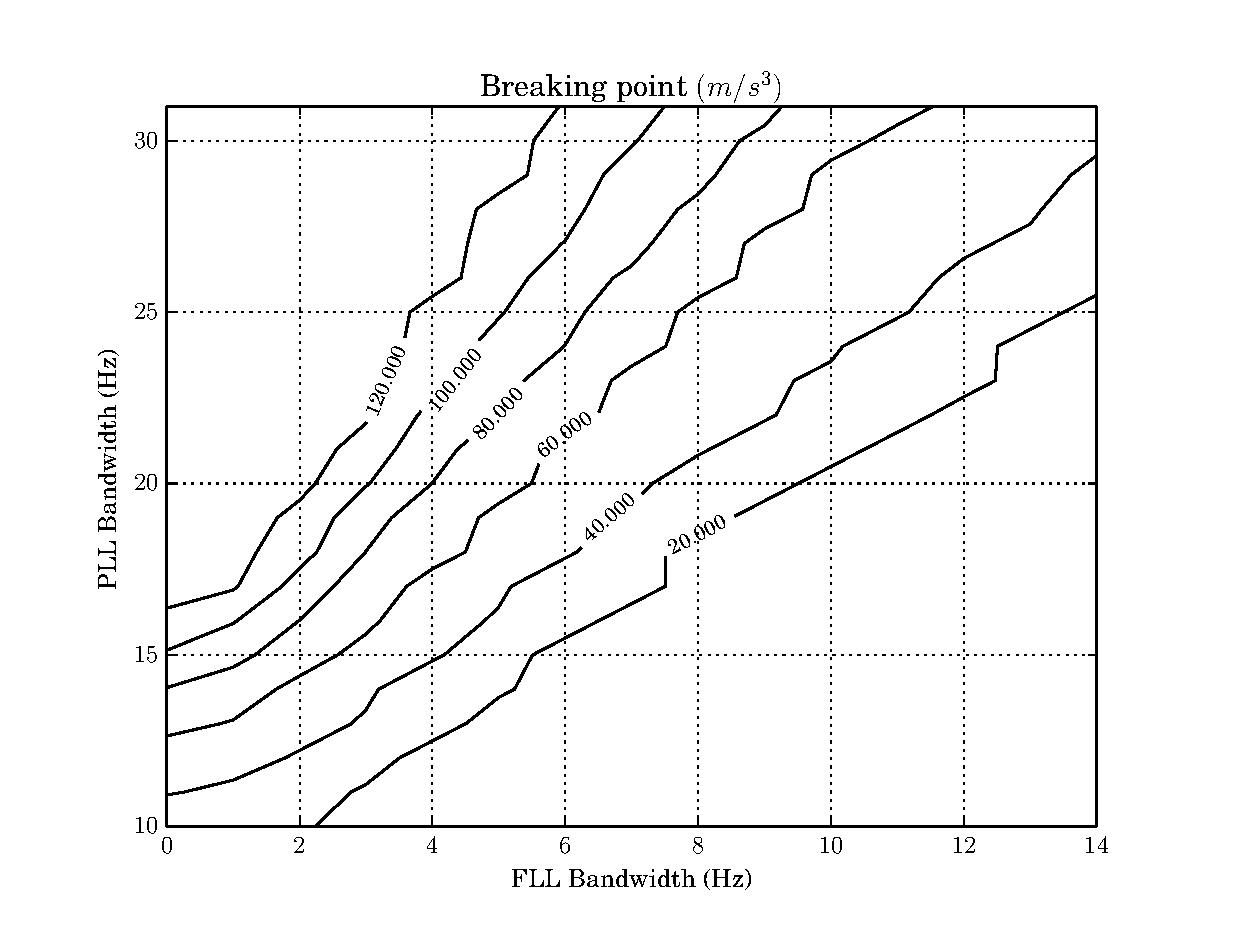
\includegraphics[width=1\textwidth]{Results/JerkContourMap.eps} 
    \caption{A contour plot of the breaking point of each PLL/FLL combination in $m/s^3$.}
    \label{fig:JerkContourMap}
\end{figure}


\begin{figure}[!htb] 
    \centering
    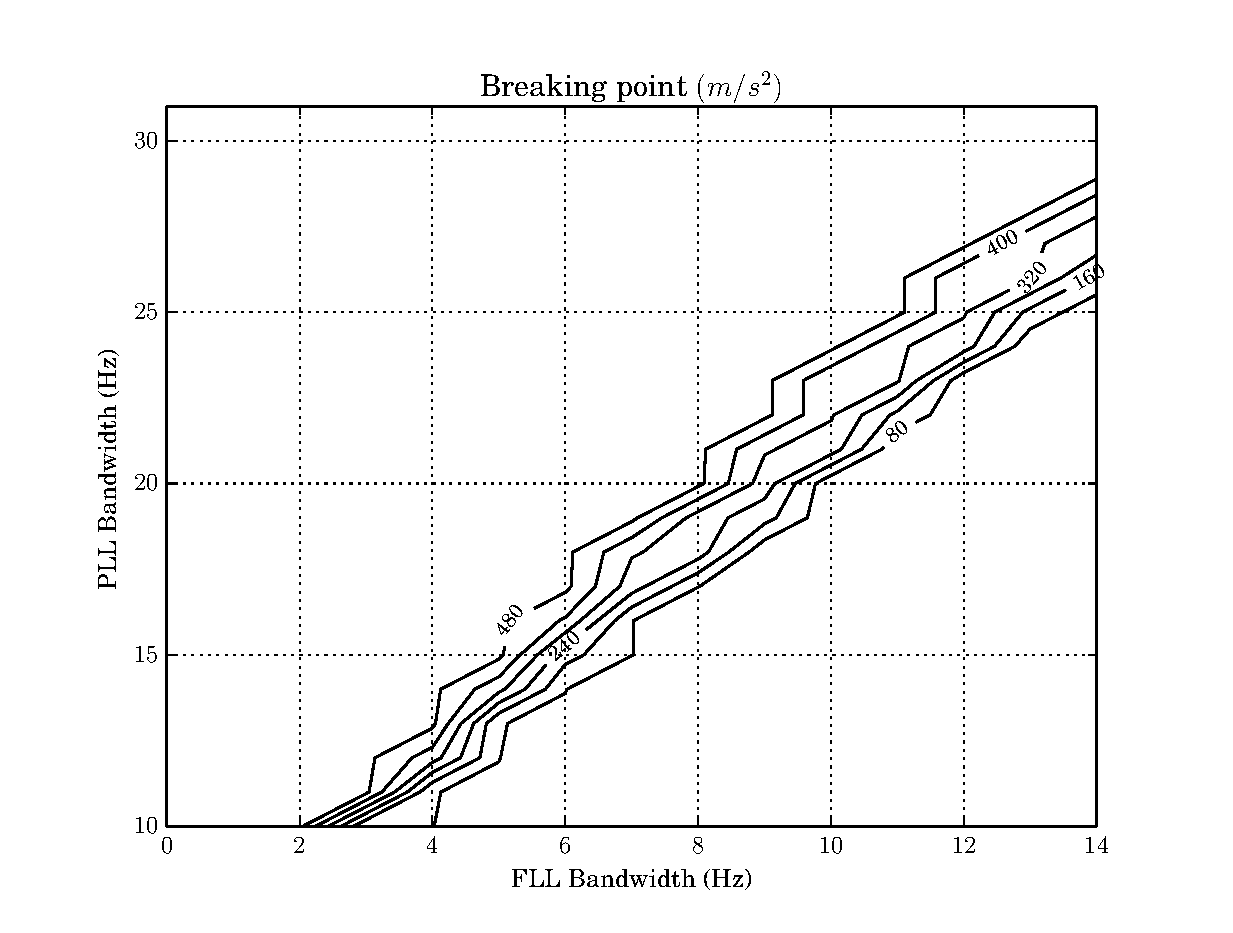
\includegraphics[width=1\textwidth]{Results/AccelerationContourMap.eps} 
    \caption{A contour plot of the breaking point of each PLL/FLL combination in $m/s^2$.}
    \label{fig:AccelerationContourMap}
\end{figure}


A Monte Carlo simulation was carried out in order to compare the performance of the existing FLL/PLL combination (1), with a loop controller with the FLL removed (2). The simulation consisted of a 200 second long ramp in jerk, as above, with the jerk increasing by 1$m/s^3$ per second. The simulation was repeated 100 times, with the breaking point and average phase being recorded. A comparison between the two loop controllers can be seen in figure \ref{fig:BoxplotJerk}. The phase jitter for the first 70 seconds was also recorded, and can be seen in figure \ref{fig:BoxplotPhaseJitter}. 

Based on the result of the Monte Carlo simulation, it is possible to conclude that the pure PLL demonstrates a significantly greater robustness with respect to jerk stresses. From a numerical perspective, the pure PLL was able to sustain operation at jerk levels  73\% higher than the combined FLL/PLL tracking loop. 

\begin{figure}[!htb] 
    \centering
    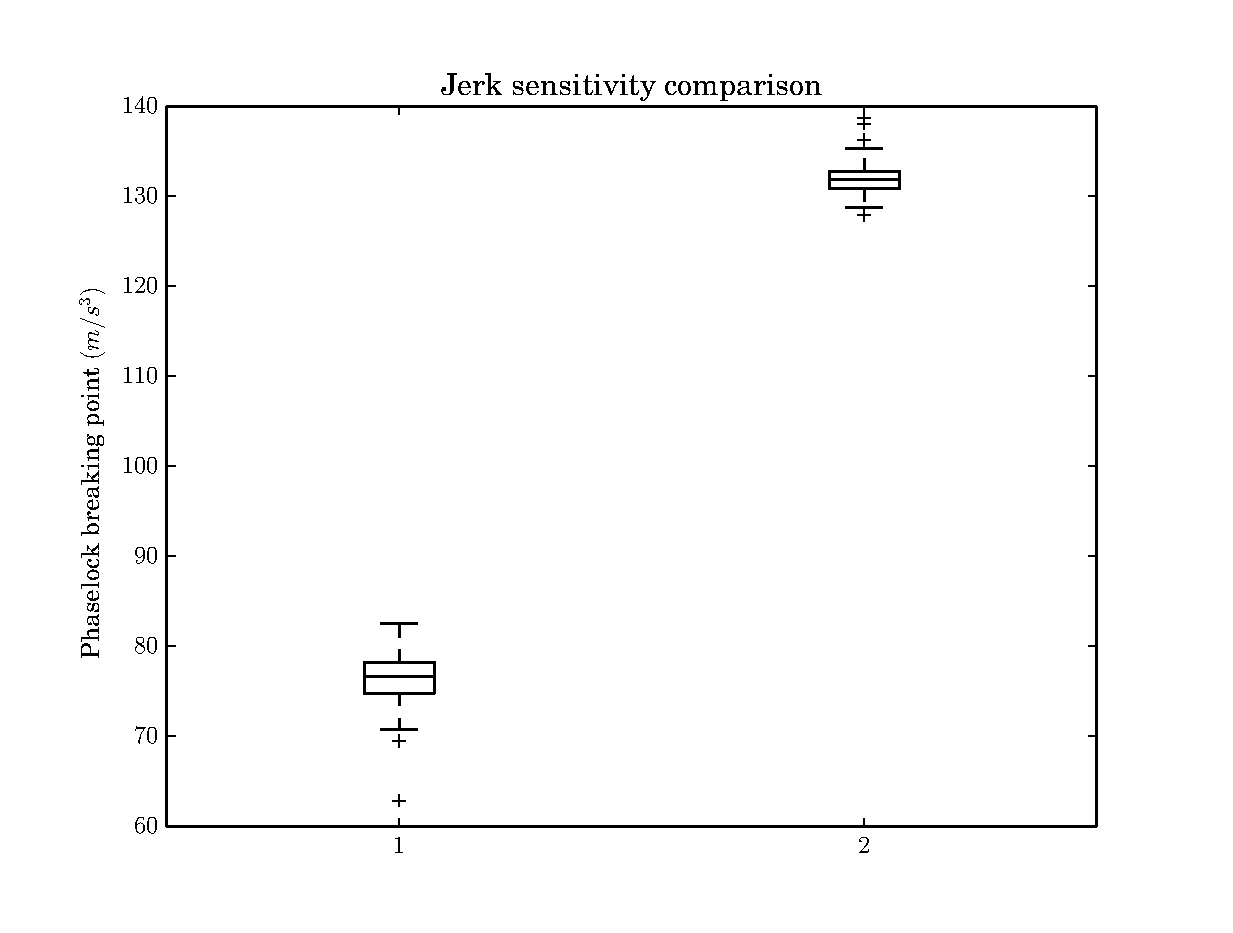
\includegraphics[width=1\textwidth]{mywork/BoxplotJerk.eps} 
    \caption{Boxplot 1 is the combined PLL/FLL, Boxplot 2 is the pure PLL. The combined PLL/FLL has an average breaking point of 76.135$\pm$2.36$m/s^3$. The pure PLL has a breaking point of 131.6 $\pm$ 1.64$m/s^3$.}
    \label{fig:BoxplotJerk}
\end{figure}

Comparing the phase jitter results from the Monte Carlo simulation, it can be ascertained that the the pure PLL demonstrates a 34\% lower phase jitter. This significant improvement helps to drive the improvements in robustness during tracking which were demonstrated in figure \ref{fig:BoxplotJerk}. 

\begin{figure}[!htb] 
    \centering
    \includegraphics[width=1\textwidth]{mywork/BoxplotPhaseJitter.eps} 
    \caption{Boxplot 1 is the combined PLL/FLL, Boxplot 2 is the pure PLL. The combined PLL/FLL has an average phase jitter of 5.78$\pm$0.28$\degree$. The pure PLL has an average phase jitter of 4.31$\pm$0.044$\degree$.}
    \label{fig:BoxplotPhaseJitter}
\end{figure}

\clearpage

\subsubsection{HighG3}

\begin{comment}
\begin{table}[!htb]
\centering
\begin{tabular}{|l|l|l|}
\hline
\rowcolor[HTML]{C0C0C0} 
SVNUM & Lock time (\%) & Phase jitter (degrees) \\ \hline
0     & 99.99 & 2.94          \\ \hline
\rowcolor[HTML]{EFEFEF} 
1     & 99.99   & 2.95          \\ \hline
3     & 99.99  & 2.95          \\ \hline
\rowcolor[HTML]{EFEFEF} 
6     & 99.99  & 2.94          \\ \hline
11    & 99.99  & 2.95          \\ \hline
\rowcolor[HTML]{EFEFEF} 
14    & 99.99  & 2.96          \\ \hline
16    & 99.99  & 2.95          \\ \hline
\rowcolor[HTML]{EFEFEF} 
18    & 99.99  & 2.94          \\ \hline
19    & 99.99  & 2.94         \\ \hline
\rowcolor[HTML]{EFEFEF} 
21    & 99.94  & 3.11         \\ \hline
22    & 99.99 & 2.94          \\ \hline
\rowcolor[HTML]{EFEFEF} 
23    & 99.99  & 2.95         \\ \hline
25    & 97.59  & 8.77          \\ \hline
\rowcolor[HTML]{EFEFEF} 
31    & 99.99  & 2.94         \\ \hline
\end{tabular}

\caption{CNO = 48,PLLBW =32,FLL=0}
\label{my-label}
\end{table}


\begin{table}[!htb]
\centering
\begin{tabular}{|l|l|l|}
\hline
\rowcolor[HTML]{C0C0C0} 
SVNUM & Lock time (\%) & Phase jitter (degrees) \\ \hline
0     & 99.99  & 4.11          \\ \hline
\rowcolor[HTML]{EFEFEF} 
1     & 99.99   & 4.10         \\ \hline
3     & 99.99  & 4.11          \\ \hline
\rowcolor[HTML]{EFEFEF} 
6     & 99.99  & 4.10          \\ \hline
11    & 99.99  & 4.12          \\ \hline
\rowcolor[HTML]{EFEFEF} 
14    & 99.99  & 4.13          \\ \hline
16    & 99.99  & 4.11         \\ \hline
\rowcolor[HTML]{EFEFEF} 
18    & 99.99  & 4.14         \\ \hline
19    & 99.99  & 4.13          \\ \hline
\rowcolor[HTML]{EFEFEF} 
21    & 99.94  & 4.18          \\ \hline
22    & 99.99  & 4.13         \\ \hline
\rowcolor[HTML]{EFEFEF} 
23    & 99.99  & 4.13          \\ \hline
25    & 97.58  & 9.22          \\ \hline
\rowcolor[HTML]{EFEFEF} 
31    & 99.99  & 4.11          \\ \hline
\end{tabular}
\caption{CNO = 48,PLLBW =32,FLL=10}
\label{my-label}
\end{table}
\end{comment}


\begin{table}[!htb]
\centering
\begin{tabular}{|l|l|l|}
\hline
\rowcolor[HTML]{C0C0C0} 
Satellite Number & Pure PLL phase jitter (degrees) & Combined PLL/FLL phase jitter (degrees) \\ \hline
1                & 2.94                            & 4.11                                    \\ \hline
\rowcolor[HTML]{EFEFEF} 
3                & 2.95                            & 4.10                                    \\ \hline
6                & 2.95                            & 4.11                                    \\ \hline
\rowcolor[HTML]{EFEFEF} 
11               & 2.94                            & 4.10                                    \\ \hline
14               & 2.95                            & 4.12                                    \\ \hline
\rowcolor[HTML]{EFEFEF} 
16               & 2.96                            & 4.13                                    \\ \hline
18               & 2.95                            & 4.11                                    \\ \hline
\rowcolor[HTML]{EFEFEF} 
19               & 2.94                            & 4.14                                    \\ \hline
21               & 2.94                            & 4.13                                    \\ \hline
\rowcolor[HTML]{EFEFEF} 
22               & 3.11                            & 4.18                                    \\ \hline
23               & 2.94                            & 4.13                                    \\ \hline
\rowcolor[HTML]{EFEFEF} 
25               & 8.77                            & 9.22                                    \\ \hline
31               & 2.94                            & 4.11                                    \\ \hline
\end{tabular}
\caption{Polaris results, $C_N/0$ = 48 dB-Hz.}
\label{tab:PolarisResultsCNO48}
\end{table}


\begin{comment}
\begin{table}[!htb]
\centering
\begin{tabular}{|l|l|l|}
\hline
\rowcolor[HTML]{C0C0C0} 
SVNUM & Lock time (\%) & Phase jitter (degrees) \\ \hline
0     & 99.99  & 5.85         \\ \hline
\rowcolor[HTML]{EFEFEF} 
1     & 99.99  & 5.87          \\ \hline
3     & 99.99  & 5.86          \\ \hline
\rowcolor[HTML]{EFEFEF} 
6     & 99.99  & 5.87          \\ \hline
11    & 99.99  & 5.87          \\ \hline
\rowcolor[HTML]{EFEFEF} 
14    & 99.99  & Lost phase-lock          \\ \hline
16    & 99.99  & 5.87          \\ \hline
\rowcolor[HTML]{EFEFEF} 
18    & 99.99  & 5.86          \\ \hline
19    & 99.99  & 5.89          \\ \hline
\rowcolor[HTML]{EFEFEF} 
21    & 99.94 & 5.90        \\ \hline
22    & 99.99  & 5.87        \\ \hline
\rowcolor[HTML]{EFEFEF} 
23    & 99.99  & 5.86          \\ \hline
25    & 59.83  & 33.34         \\ \hline
\rowcolor[HTML]{EFEFEF} 
31    & 99.99  & 5.86          \\ \hline
\end{tabular}
\caption{CNO = 42,PLLBW =32,FLL=0}
\label{my-label}
\end{table}

\begin{table}[!htb]
\centering
\begin{tabular}{|l|l|l|}
\hline
\rowcolor[HTML]{C0C0C0} 
SVNUM & Lock time (\%) & Phase jitter (degrees) \\ \hline
0     & 99.991  & 8.23         \\ \hline
\rowcolor[HTML]{EFEFEF} 
1     & 99.99  & 8.23        \\ \hline
3     & 99.99  & 8.22          \\ \hline
\rowcolor[HTML]{EFEFEF} 
6     & 99.99  & 8.21         \\ \hline
11    & 99.99  & 8.22         \\ \hline
\rowcolor[HTML]{EFEFEF} 
14    & 99.99  & 8.22         \\ \hline
16    & 99.99  & 8.22           \\ \hline
\rowcolor[HTML]{EFEFEF} 
18    & 99.99  & 8.21          \\ \hline
19    & 99.99  & 8.24          \\ \hline
\rowcolor[HTML]{EFEFEF} 
21    & 99.94  & 8.26          \\ \hline
22    & 99.99  & 8.2          \\ \hline
\rowcolor[HTML]{EFEFEF} 
23    & 99.99  & 8.23         \\ \hline
25    & 43.58  & 39.65          \\ \hline
\rowcolor[HTML]{EFEFEF} 
31    & 99.99  & 8.22         \\ \hline
\end{tabular}
\caption{CNO = 42,PLLBW =32,FLL=10}
\label{my-label}
\end{table}
\end{comment}


\begin{table}[!htb]
\centering
\begin{tabular}{|l|l|l|}
\hline
\rowcolor[HTML]{C0C0C0} 
Satellite Number & Pure PLL phase jitter (degrees) & Combined PLL/FLL phase jitter (degrees) \\ \hline
1                & 5.87                            & 8.23                                    \\ \hline
\rowcolor[HTML]{EFEFEF} 
3                & 5.85                            & 8.22                                    \\ \hline
6                & 5.86                            & 8.21                                    \\ \hline
\rowcolor[HTML]{EFEFEF} 
11               & 5.87                            & 8.22                                    \\ \hline
14               & 5.86                            & 8.22                                    \\ \hline
\rowcolor[HTML]{EFEFEF} 
16               & 5.87                            & 8.22                                    \\ \hline
18               & 5.86                            & 8.21                                    \\ \hline
\rowcolor[HTML]{EFEFEF} 
19               & 5.89                            & 8.24                                    \\ \hline
21               & 5.90                            & 8.26                                    \\ \hline
\rowcolor[HTML]{EFEFEF} 
22               & 5.87                            & 8.20                                    \\ \hline
23               & 5.86                            & 8.23                                    \\ \hline
\rowcolor[HTML]{EFEFEF} 
25               & 33.4                            & 39.65                                   \\ \hline
31               & 5.86                            & 4.11                                    \\ \hline
\end{tabular}
\caption{Polaris results, $C_N/0$ = 42 dB-Hz.}
\label{tab:PolarisResultsCNO42}
\end{table}




\clearpage
\subsection{Hardware simulation}

\subsubsection{HighG3}


\begin{comment}
\begin{table}[!htb]
\centering
\begin{tabular}{|l|l|l|}
\hline
\rowcolor[HTML]{C0C0C0} 
Channel number & Satellite number & Phase jitter       \\ \hline
0              & 3                & 7.09 \\ \hline
\rowcolor[HTML]{EFEFEF} 
1              & 6                & 7.18 \\ \hline
2              & 11               & 7.11 \\ \hline
\rowcolor[HTML]{EFEFEF} 
3              & 14               & 7.12 \\ \hline
4              & 16               & 6.87 \\ \hline
\rowcolor[HTML]{EFEFEF} 
5              & 18               & 5.68 \\ \hline
6              & 19               & 7.14  \\ \hline
\rowcolor[HTML]{EFEFEF} 
7              & 22               & 7.15 \\ \hline
\end{tabular}
\caption{CNO = 48,PLLBW =32,FLL=0}
\label{my-label}
\end{table}




\begin{table}[!htb]
\centering
\begin{tabular}{|l|l|l|}
\hline
\rowcolor[HTML]{C0C0C0} 
Channel number & Satellite number & Phase jitter       \\ \hline
0              & 14               & 5.37 \\ \hline
\rowcolor[HTML]{EFEFEF} 
1              & 3                & 9.16 \\ \hline
2              & 6                & 9.21 \\ \hline
\rowcolor[HTML]{EFEFEF} 
3              & 18               & 9.35 \\ \hline
4              & 11               & 9.11 \\ \hline
\rowcolor[HTML]{EFEFEF} 
5              & 16               & 9.06 \\ \hline
6              & 19               & 9.07 \\ \hline
\rowcolor[HTML]{EFEFEF} 
7              & 22               & 7.89 \\ \hline
\end{tabular}
\caption{CNO = 42,PLLBW =32,FLL=0}
\label{my-label}
\end{table}
\end{comment}


\begin{table}[!htb]
\centering
\begin{tabular}{|l|l|l|}
\hline
\rowcolor[HTML]{C0C0C0} 
Satellite Number & Pure PLL phase jitter (degrees) & Combined PLL/FLL phase jitter (degrees) \\ \hline
3                & 7.09                            & Lost phase-lock                               \\ \hline
\rowcolor[HTML]{EFEFEF} 
6                & 7.18                            & 9.16                                    \\ \hline
11               & 7.11                            & 9.21                                    \\ \hline
\rowcolor[HTML]{EFEFEF} 
14               & 7.12                            & 9.35                                    \\ \hline
16               & 6.87                            & 9.11                                    \\ \hline
\rowcolor[HTML]{EFEFEF} 
18               & Lost phase-lock                          & 9.06                                    \\ \hline
19               & 7.14                            & 9.07                                    \\ \hline
\rowcolor[HTML]{EFEFEF} 
22               & 7.15                            & Lost phase-lock                               \\ \hline
\end{tabular}
\caption{Spirent results, $C_N/0$ = 48 dB-Hz.}
\label{tab:SpirentCNO48}
\end{table}


\begin{table}[!htb]
\centering
\begin{tabular}{|l|l|l|}
\hline
\rowcolor[HTML]{C0C0C0} 
Channel number & Satellite number & Pure PLL phase jitter (degrees)      \\ \hline
0              & 3                & 7.72 \\ \hline
\rowcolor[HTML]{EFEFEF} 
1              & 22               & 7.70 \\ \hline
2              & 18               & 6.98\\ \hline
\rowcolor[HTML]{EFEFEF} 
3              & 6                & 7.73 \\ \hline
4              & 16               & 7.73 \\ \hline
\rowcolor[HTML]{EFEFEF} 
5              & 14               & Lost phase-lock \\ \hline
6              & 19               & 7.70 \\ \hline
\rowcolor[HTML]{EFEFEF} 
7              & 11               & 7.68 \\ \hline
\end{tabular}
\label{tab:SpirentCNO42}
\caption{Spirent results, $C_N/0$ = 48 dB-Hz.}
\end{table}




\clearpage
\subsection{Discussion}




